\section{Analysis Overview}
\label{sec:analysis_overview}
The first step to performing a precision measurement of the Higgs boson mass (\mH) is to ``observe'' many Higgs bosons.
However, production of a Higgs boson is essentially nonexistent in everyday conditions and is still extremely rare even in the high-energy \pp collisions of the LHC.
Even at the center-of-mass energy of 13\TeV, the total inclusive inelastic cross section of two protons colliding is 70\mb TODO: CITE.
Comparing this to the production cross section of a Higgs boson (TODO sigma(pptoH) = 59 pb) shows that a Higgs boson is produced in approximately only 1 out of about every billion \pp collisions.  TODO CITE

To complicate matters further, the Higgs boson has a \emph{very} short mean lifetime of only $1.6 \tentotheminus{22}\snd$~\cite{pdg}.
Thus, the Higgs boson is not directly detected by CMS but is instead \emph{inferred} from via the stable decay products enter the various subdetectors.


Higgs boson decays via variety of decay modes.
Look at Figure to see branching ratios/fractions.



Real particles enter detectors in CMS which send signals to various electronics.
Particle Flow algorithm pieces the information together to construct objects out of each event.
Now, instead of just a deposit of energy in the ECAL and corresponding hits in the silicon tracker, the particle is identified as a newly produced electron.
CMS records which kinds of objects came from which events and stores the information in \emph{data sets} (TODO: ref Section future).
Since there is an enormous amount of data to sift through, analysts can look at which events caused which \emph{triggers} (TODO: ref Section previous cms triggers)

Using special triggers
%~\ref{}
that sort events

It is therefore imperative to collect as many signal events as possible.

This is achieved by careful event selection from the physics objects stored within the CMS data sets.

Unfortunately, the \hzzfourl process is rare because 
This is done by sifting through \pp collision data analyzed by the CMS detector (Chapter~\ref{ch:cms_detector}) to identify all possible \hzzfourl events (the \emph{signal} process).
This signal process is used because it has a large signal-to-background ratio of approximately 2.
Furthermore, even if a Higgs boson is produced, it decays into two \PZ bosons only 2.6\% of the time (Figure~\ref{fig:higgs_br}).
\begin{figure}[!htbp]
    \begin{center}
        % Figures come from:
        % https://twiki.cern.ch/twiki/bin/view/LHCPhysics/LHCHWG?redirectedfrom=LHCPhysics.LHCHXSWG#Higgs_cross_sections_and_decay_b
		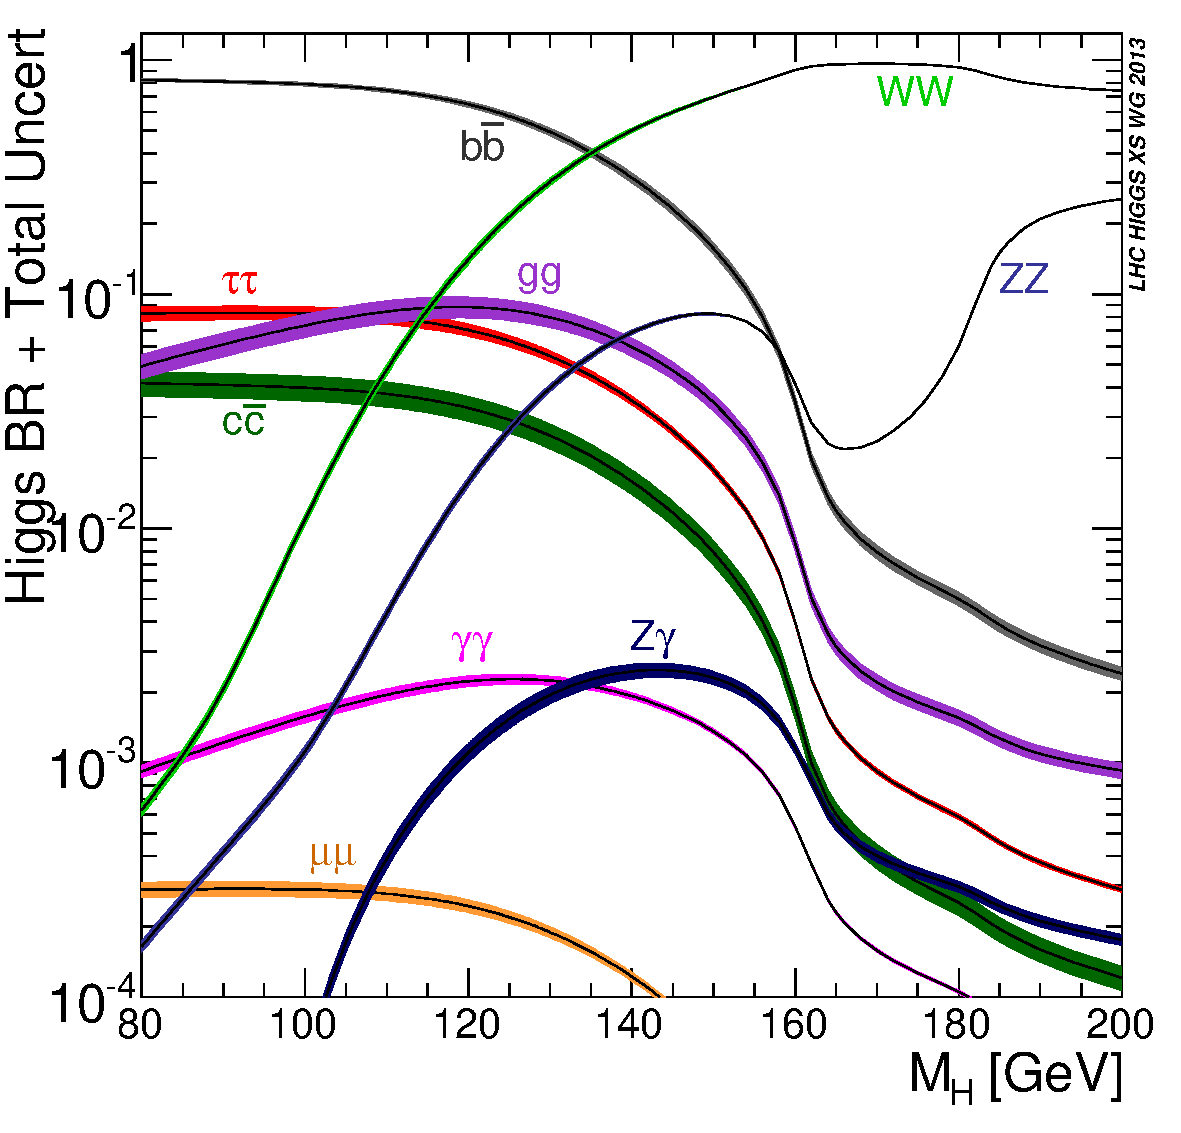
\includegraphics[width=0.48\textwidth]{figures/higgsmassmeas/higgs_BR_80to200GeV.pdf}
		\includegraphics[width=0.48\textwidth]{figures/higgsmassmeas/higgs_BR_120to130GeV.pdf}
		\caption{The branching ratios of various Higgs boson decays as a function of the Higgs boson mass.}
		\label{fig:higgs_br}
	\end{center}
\end{figure}
This percentage is typically expressed as a fraction, called the \emph{branching fraction} or \emph{branching ratio} (\br).
Those \PZ bosons then decay into opposite-sign, same flavor leptons (\Ztolplm, where $\ell = \Pe, \mu$) only 6.7\% of the time, making the branching ratio of the signal process approximately: % B(Z->ee)=0.033632, B(Z->mumu)=0.033662
\begin{equation*}
    \BRof{\hzzfourl} = \BRof{\htozz} \left[ \BRof{\Ztolplm} \right]^2 = 1.8\tentotheminus{3}.
\end{equation*}
Thus, the signal process is produced only once about every \emph{trillion} \pp collisions.


- By collecting events with the \fourl final state, we are likely to find signal events.
    - It's not just the signal process which produces \fourl: background also makes \fourl (Section FIXME).
- Before analyzing the data, however, it is important to make predictions using simulated samples (Section FIXME).
- In order to sort signal from background, use simulated samples 



, which is the formation of particle physics objects from data.
The data collected and analyzed by CMS is not so simple so as to have \htozz


This process hinges on the conservation of momentum, since in the longitudinal ($z$) direction the \pp collision has initial and final.
Specifically, the 
    - The \PZ boson has a precisely measured mass of TODO a neutral particle, so the two leptons into which it decays should combine to Group two leptons together, 
    - Form two different pairs of opposite-sign, same-flavor (OSSF) leptons
    - If it appears that the to select specific hzz4l events (\emph{event selection}).

